\documentclass[11pt]{article}

\usepackage{amsmath}
\usepackage{amssymb}
\usepackage{bbm}
\usepackage{booktabs}
\usepackage{natbib}
\usepackage{color}
\usepackage{caption}
\newcommand\fnote[1]{\captionsetup{font=scriptsize}\caption*{\textsl{Note:} #1}}
\newcommand\fnotes[1]{\captionsetup{font=scriptsize}\caption*{\textsl{Notes:} #1}}
\usepackage{float, afterpage, rotating, graphicx}% Including fig and tab
\usepackage{epstopdf}% Convert eps to pdf, graphicx needs to be loaded before
\usepackage{hyperref}

\title{Whitepaper: LCI 20}
\author{
Onno Kleen\thanks{Heidelberg University, Department of Economics, \href{mailto:onno.kleen@awi.uni-heidelberg.de}{onno.kleen@awi.uni-heidelberg.de}}
\and
Christopher Zuber\thanks{Heidelberg University, Department of Economics, \href{mailto:christopher.zuber@awi.uni-heidelberg.de}{christopher.zuber@awi.uni-heidelberg.de}}
}
\begin{document}
\maketitle
\section{Outline}

We propose the Lykke Crypto Index 20 (LCI 20) to be a weighted average of the 20 largest crypto currencies' market capitalization.\footnote{Code and .tex-files can be found at \href{https://github.com/onnokleen/crypto-index}{https://github.com/onnokleen/crypto-index}}
The purpose of our index is to closely follow the value of crypto-currencies in comparison to the US dollar.
We address crypto-currency-specific problems as there are
For example, the distinct market behavior around currency-splits is addressed by adaptively smoothing prices of affected assets.

In comparison to \cite{Trimborn2016}, we choose keeping the amount of assets included to be fixed.
This has the advantage of interpreting currencies included being among the 20th most ``important'' crypto-assets.

We procede as follows: 
First, notation and our index calculation are introduced. 
Second, we discuss pros and cons of our method.
Third, a reduced-form example of our index on daily data is presented.

\subsection{Definition}

Let $t$ denote our (possibly continuous) time index starting at time $t_0$.
Moreover, $\mathcal{C}_t \in \mathbb{N}$ is the set of coins that are tradable at time $t$ across $M \in \mathbb{N}$ relevant market places for crypto-assets.
The price of asset $i$ at time $t$ is calculated as the mean of the bid-ask spread's midpoint across all $M$ markets.
Quantity $q_{i,t}$ denotes the overall number of currently mined shares/items of asset $i$ at time $t$.
Last, we need a measure of market capitalization $c_{i,t}$.
Whereas $p_{i,t}$ and $q_{i,t}$ are ``hard facts'', market capitalization is a more vague term.

\begin{figure}%
    \centering%
    \caption{Evolution of LCI20}\label{f:lci20}%
    %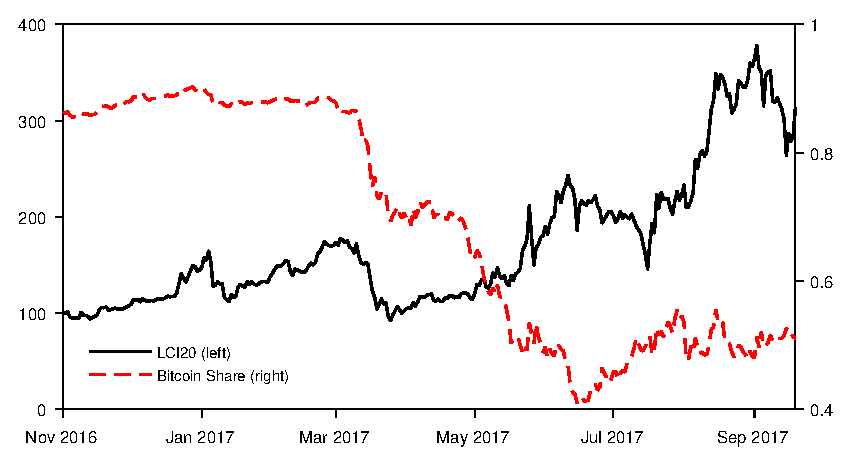
\includegraphics[width=\textwidth]{../bld/figures/lci20.eps}%
    \fnotes{Put notes here.}
    % \medskip\newline% Separate caption and notes
    % \begin{minipage}{\textwidth}
        % {\scriptsize \textit{Note:} Put notes here.\par}
    % \end{minipage}
\end{figure}

In stock market indices, only shares that are actively tradable, called the ``public float'' are included in calculating those indices by excluding shares held by strategic long-term investors, e.g.\ founding shareholders or government.
As there is no public recording to which person or institutions long-term

Our index can be interpreted as a standardized ratio of weighted sums relative to its initial value. 

\subsection{Six steps for calculating LCI 20}

Our index is defined as a standardized ratio of weighted sums relative to its initial value:
\begin{equation}
  \text{LCI20}_t = 100 * \frac{\widetilde{\text{LCI20}}_t}{\widetilde{\text{LCI20}}_{t_0}}
\end{equation}

\begin{enumerate}
  \item Calculate each coins market share $s_{i,t}$.
  \item Truncate market shares by maximum $\bar s$: $\bar s_{i,t} = \max\{ s_{i,t}, \bar s\}$
  \item Rescale them, so weights sum up to one: $w_{i,t} = \frac{\bar s_{i,t}}{\sum_{i \in \mathcal{C}_t} \bar s_{i,t}}$. %Note that $w_{i,t}$ is afterwards greater than $0.25$ due to rescaling.
  \item Calculate the weighted average $$\widetilde{\text{LCI20}}_t = \sum_{i \in \mathcal{C}_{t}} w_{i,t} c_{i,t}$$
  \item The initial value of the weighted sum is given by $$\widetilde{\text{LCI20}}_{t_0} = \sum_{i \in \mathcal{C}_{t}} w_{i,t_0} c_{i,t_0}$$
  \item $Divisor = \widetilde{\text{LCI20}}_{t_0}$
\end{enumerate}


\begin{figure}%
    \centering%
    \caption{LCI20 vs.\ bitcoin price}\label{f:lci20vsBTC}%
    %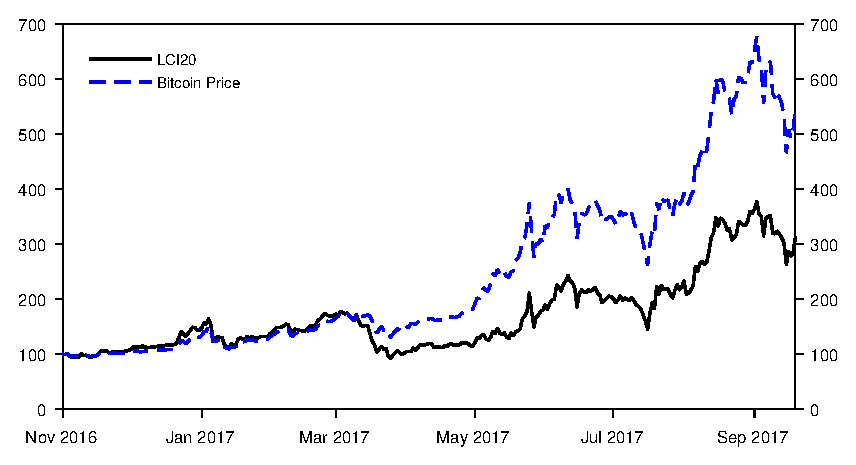
\includegraphics[width=\textwidth]{../bld/figures/lci20_vs_btc.eps}%
    % \medskip\newline% Separate caption and notes
    \fnotes{Put notes here.}
    % \begin{minipage}{\textwidth}
        % {\scriptsize \textit{Note:} Put notes here.\par}
    % \end{minipage}
\end{figure}

\begin{figure}%
    \centering%
    %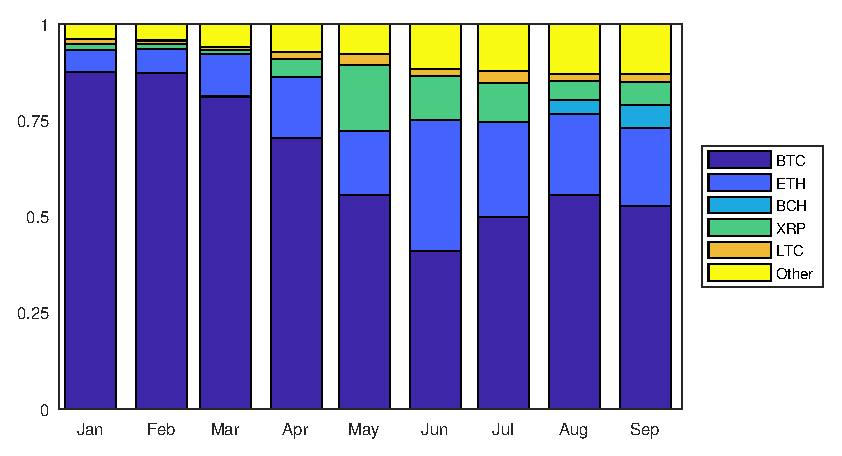
\includegraphics[width=\textwidth]{../bld/figures/currency_shares.eps}%
    \caption{Currency shares along 2017}\label{f:curshares}%
    %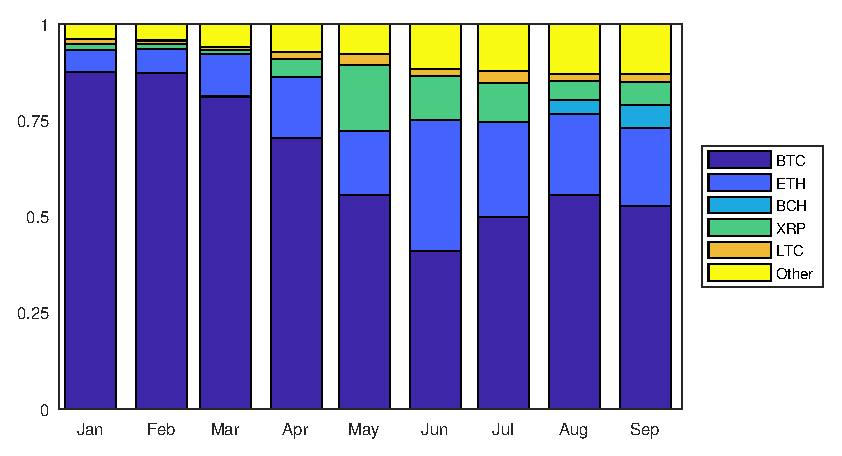
\includegraphics[width=\textwidth]{../bld/figures/currency_shares.eps}%
    % \medskip\newline% Separate caption and notes
    \fnotes{Some notes}
    % \begin{minipage}{\textwidth}
        % {\scriptsize \textit{Note:} Put notes here.\par}
    % \end{minipage}
\end{figure}

\subsection{Addressing splits}\label{subseq:split_smoothing}
For anticipated splits/forks we propose an adaptive smoothing technique for addressing ``insane'' price movements in direct aftermath.
We propose to use one-hour averaged prices for currencies that are anticipated to split when calculating LCI20 beginning one day in advance and ending one day after split 


\subsection{Questions to address}
\begin{itemize}
  \item Why 20 currencies? 19-09-2017 14:41 20th market capitalization (STEEM) is only \$286.382.955 and 24 hour trading volume of \$686. Further, the 20 currencies with the highest market capitalization have a share of 92 \% of the total market capitalization and a 24 hour trading volume of 94 \% of the total trading volume of September 22, 2017. If we add another 30 currencies, the 24 hour trading volume increases by 2 percentage points where we think that a smaller but better traceable index outweighs an index with a larger but more volatile currency base.
  \item ``Dead coins'' a problem?
  \item If there is a split (like Bitcoin), new currency is part of Lykke 20 but is part of constituents-check at the end of the week.
  \item Basis: 100 Punkte?
  \item How to get market capitalization of public float?
  \item Maximal weight maybe 20\%? DAX: Maximum weight 10\%.
\end{itemize}

Wikipedia:  In general, the large holdings of founding shareholders, corporate cross-holdings, and government holdings in partially privatized companies are excluded when calculating the size of a public float.

https://www.coindesk.com/rethinking-bitcoin-market-cap/: In 2014, NVIDIA engineer John Ratcliff theorized that approximately 30\% of the current bitcoin supply is made up of ``zombie'' bitcoins that have been inactive for more than a year This number includes bitcoins connected to inaccessible wallets, government-seized bitcoins, ``burned'' bitcoins and bitcoins abandoned during the early days of bitcoins, including Nakamoto's mythical stash of over a million bitcoins.

\subsection{How does it work in other indices}

\begin{itemize}
  \item DAX: Weighting based on market capitalization of public float (bedeutet Streubesitz, keine Aktien von Langzeitanlegern  wie Familie Porsche/Quant).
\end{itemize}

\subsection{Features}

\begin{itemize}
  \item
  \item Constituent changes each week. Maybe Friday? Maybe based on trade volume in last 7 days? Good against ``dead coins''.
\end{itemize}

\begin{table*}
\caption{Table explaining differences: proposal vs.\ example}
\centering
\resizebox{\textwidth}{!}{
\begin{tabular}{ccc}
  Issue & Our Proposal & Example \\
  \midrule
  Frequency & Real-time & Daily \\
  Split-smoothing & See Subsection \ref{subseq:split_smoothing} & Not necessary due to daily data\\
  Public float & Only use coins that have been traded the last 4 years - weekly updated (real-time tracking difficult) & nothing \\
  ``Zombie coins'' & Only use coins that have been traded the last 4 years & only use 0.30\%\\
\bottomrule
\end{tabular}
}
\fnotes{In this table differences in implementation of our example and our actual proposal are reported.}
\end{table*}

\section{Discussion}

Immaturity of market may lead right now to frequent changes of assets included in the lower ranks of our index.
However, we want our definition of the LCI 20 to be ``future-proof'' and expect volatility among ranking of crypto-assets in terms of market capitalization should to decrease in the upcoming two years.


\section{Example: Daily LCI 20}

\subsection{Data}

We download daily closing prices and market capitalization from \href{https://coincap.com}{coincap.com} via their Rest API.
Our data set includes up to x different cryptocurrencies listed on \href{https://coincap.com}{coincap.com} in between .2017 and 19.09.2017.\footnote{Currencies are included if they were among the currencies with the largest market capitalization at \dots}


Something nice to illustrate:
\begin{itemize}
  \item Volatility in August (Bitcoin-split versus July). Show new composition after split.
\end{itemize}

\section{Splits}

The volatility of the index increases in times shortly before and after a split.
For example, the index dropped on August 2, 2017, the day after the hard fork of Bitcoin Cash by $-12.7$ \% which is due to the price drop of Bitcoin ($-5$ \%) and the lower price of Bitcoin Cash (roughly 1/6 of Bitcoin).
At this point, investors which held Bitcoin, get the same amount of Bitcoin Cash.
However, both currencies share the same transaction history.
If one incautiously pushes now a transaction containing only old coins to the wrong transaction chain, one will loese the pushed value in both currencies.
Therefore, private investors are usually advised not to trade their old coins or newly gained currency in the days after a split but to wait until it is settled if the new currency becomes accepted.


\begin{figure}%
    \centering%
    %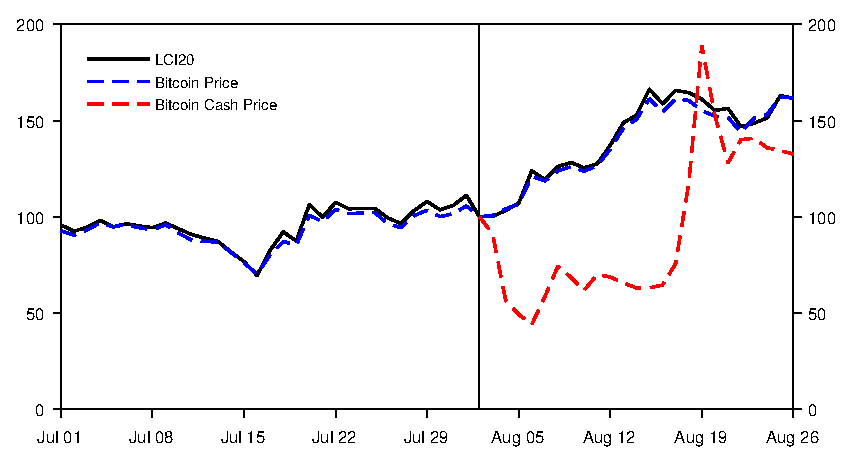
\includegraphics[width=\textwidth]{../bld/figures/lci20_bch_split.eps}%
    \caption{LCI20 at Bitcoin Cash split}\label{f:split}%
    % \medskip\newline% Separate caption and notes
    % \begin{minipage}{\textwidth}
        % {\scriptsize \textit{Note:} Put notes here.\par}
    % \end{minipage}
\end{figure}



\bibliographystyle{ecca}
\bibliography{crypto-index}

\end{document}
